% Clean CV/Resume Template, by Bennet B <dev@bennet.cc>
% CC0, Public-Domain
% 
% Permission is hereby granted, free of charge, to any person obtaining a copy
% of this template and associated files (the "Template"), to deal
% in the Template without restriction, including without limitation the rights
% to use, copy, modify, merge, publish, distribute, sublicense, and/or sell
% copies of the Template, and to permit persons to whom the Template is
% furnished to do so, subject to the following conditions:
%
% The above copyright notice and this permission notice shall be included in all
% copies or substantial portions of the Template.
%
% THE TEMPLATE IS PROVIDED "AS IS", WITHOUT WARRANTY OF ANY KIND, EXPRESS OR
% IMPLIED, INCLUDING BUT NOT LIMITED TO THE WARRANTIES OF MERCHANTABILITY,
% FITNESS FOR A PARTICULAR PURPOSE AND NONINFRINGEMENT. IN NO EVENT SHALL THE
% AUTHORS OR COPYRIGHT HOLDERS BE LIABLE FOR ANY CLAIM, DAMAGES OR OTHER
% LIABILITY, WHETHER IN AN ACTION OF CONTRACT, TORT OR OTHERWISE, ARISING FROM,
% OUT OF OR IN CONNECTION WITH THE TEMPLATE OR THE USE OR OTHER DEALINGS IN THE
% TEMPLATE.
%
% based on Modern CV by Habib Semouma
% https://www.overleaf.com/latex/templates/modern-cv-slash-resume-template/vjrqdkpjckwj
%
%
% !TEX program = XeLaTeX
\documentclass[onside]{article}

\usepackage{wallpaper}
\usepackage{geometry}
\usepackage[
    unicode=true,
    bookmarks=true,
    bookmarksnumbered=false,
    bookmarksopen=true,
    bookmarksopenlevel=1,
    breaklinks=false,
    pdfborder={0 0 0},
    backref=false,
    colorlinks=false
    ]{hyperref}
\usepackage{lastpage}
\usepackage{hyphenat}
\usepackage{hyphsubst}
\usepackage{tabularx}
\usepackage{moresize}
\usepackage[document]{ragged2e}
% \usepackage{parskip}
\usepackage[scaled]{helvet}
\usepackage{nopageno}
\usepackage{fontawesome5}
\usepackage{fontawesome}
\usepackage{academicons}
\usepackage[defaultfam,tabular,oldstyle]{montserrat}
\usepackage[T1]{fontenc}
\usepackage[utf8]{inputenc}
\usepackage[english,german]{babel}
%\usepackage{lmodern}

%\usepackage{afterpage}
\renewcommand*\oldstylenums[1]{{\fontfamily{Montserrat-TOsF}\selectfont #1}}
\usepackage{graphicx}
\usepackage{titlesec}
\usepackage{xcolor}
\usepackage{tikz}
\usepackage{color}
\usepackage{amsmath}

\setlength{\parindent}{0pt}
\titleformat{\section}{\normalfont}{}{0pt}{}

\renewcommand{\arraystretch}{1.4}

\setlength\fboxrule{0pt}
\setlength\fboxsep{12pt}
% \setlength{\parskip}{.5\baselineskip plus 2pt}
% \renewcommand{\baselinestretch}{1.1}
%\enlargethispage{-\baselineskip}
\titlespacing{\section}{0pt}{1.5ex plus .1ex minus .2ex}{1pc}

\newcolumntype{Y}{>{\RaggedRight\arraybackslash}X}

% Change PDF Meta Info here
\hypersetup{
    pdftitle={Morteza Montahaee - CV - English/German},
    pdfauthor={Morteza Montahaee},
    pdfsubject={CV},
    pdftitle={Mein CV erstellt mit LaTeX},
%    pdfpagemode=FullScreen,
}

% Paper size
\geometry{
    a4paper,
    left=0pt,
    right=0pt,
    top=0pt,
    bottom=0pt,
    nohead,
    % includefoot,
    nomarginpar
}

% Background Color of the Sidebar Column
\definecolor{sidebg}{cmyk}{1, 0.02, 0, 0.56}
% Background Color of the Main Column
\definecolor{mainbg}{cmyk}{0, 0, 0.07, 0.04}

% Text Color of the Main Column
\definecolor{maintext}{cmyk}{1, 0.02, 0, 0.8}
% Text Color of the Sidebar Column
\definecolor{sidetext}{cmyk}{0, 0, 0.07, 0.04}
\definecolor{bgcol}{RGB}{115,115,115}
\definecolor{darkgreen}{RGB}{0,110,0}

\pagecolor{mainbg}

%%%%%%%%%%%%%%%%%%%%%%%%%%%%%%%%%%%%%%%%%%%%%%%%%
% Your newcommands
\newcommand{\eduevent}[5]{
        {\scshape\fontseries{light}\selectfont\footnotesize \faMapMarker{} #1 \qquad{} \faCalendar{} #2 \textendash{} #3} \\
}
\renewcommand{\eduevent}[6]{
%    \begin{tabularx}{\linewidth}{@{}X@{\hspace{-2.5cm}}r@{}}
    \begin{tabularx}{\linewidth}{@{}l@{\hspace{#6}}Xr@{}}
    {\scshape\fontseries{light}\selectfont\footnotesize \scalebox{1.144}{\faMapMarker}{} #1} & {\scshape\fontseries{light}\selectfont\footnotesize \faCalendar{} #2 \textendash{} #3} \\
    {{#4:} & {#5}} \\[1ex]
    \end{tabularx}
}

\newcommand{\jobevent}[5]{%
    \begin{tabularx}{\linewidth}{@{}l@{\hspace{#5}}Xr@{}}%
    {\scshape\fontseries{light}\selectfont\footnotesize \scalebox{1.144}{\faMapMarker}{} #1} & {\scshape\fontseries{light}\selectfont\footnotesize \faCalendar{} #2 \textendash{} #3} \\
    {#4} \\[1ex]%
    \end{tabularx}%
}

\newcommand{\betiny}{\fontsize{6pt}{7pt}\selectfont}

\newcommand{\externallink}[2]{
    \href{#1}{\scalebox{#2}{\faExternalLink}}
}

\renewcommand{\externallink}[3]{%
    \ifthenelse{\equal{#3}{true}}{%
    % Superscript (raised) version
        \href{#1}{$^{\scalebox{#2}{\faExternalLink}}$}%
    }{%
    % Normal version
        \href{#1}{\scalebox{#2}{\faExternalLink}}%
    }%
}


\renewcommand{\externallink}[5]{%
    \href{#1}{\raisebox{{#3}ex}{\hspace{{#4}em}\rotatebox{#5}{\scalebox{#2}{\faExternalLink}}}}%
}

\newcommand{\internallink}[5]{%
    \href{#1}{\raisebox{{#3}ex}{\hspace{{#4}em}\rotatebox{#5}{
\includegraphics[width={#2}em]{internalLink}}}%
    }
}


% a six pointed arrow poiting to the left
\newcommand{\tzlarrow}{(0,0) -- (0.2,0) -- (0.3,0.2) -- (0.2,0.4) -- (0,0.4) -- (0.1,0.2) -- cycle;}

% include the left arrow into a tikz picture
% param1: fill color
%
\newcommand{\larrow}[1]{
    \begin{tikzpicture}[scale=0.65]
    %\begin{tikzpicture}{justify}[scale=0.58]
    \filldraw[fill=#1!80,draw=#1!80!black]  \tzlarrow
    \end{tikzpicture}
}

% creates a stretched box as cv entry detail
% param 1:	information describing the event
%
\newcommand{\cvdetail}[1]{
    \begin{tabular*}{1\textwidth}{p{2.56cm} p{14.44cm}}
    & \larrow{bgcol}  #1\\ [3pt]
    \end{tabular*}
}
%\pdfpageattr{/AA << /O << /S /JavaScript /JS (this.zoom = 125) >> >>}

\begin{document}
\setlength{\topskip}{0pt}\setlength{\footskip}{0pt}%
\fcolorbox{red}{sidebg}{%
    \begin{minipage}[t][\textheight-2\fboxsep-2\fboxrule][t]{\dimexpr0.40\textwidth-2\fboxrule-2\fboxsep\relax}
        \color{sidetext}
        %%%%%%%%%%%%%%%%%%%%%%%%%%%%%%%%%%%%%%%%%%%%%%%%%%%%
        % YOUR NAME, PRONOUNS, OCCUPATION(s), AND HEADSHOT
        {\bfseries\scshape\HUGE Morteza} \\
        {\bfseries\scshape\huge Monthaee} \qquad {\large\textbf{ Lebenslauf}}
        \vspace{.3cm} \\
        % Demo Subject, \\
        {\faStarOfLife{}  17/09/1984}
        \\
        \begin{center}
            \begin{tikzpicture}
            \clip (0,0) circle (3cm) node[anchor=center] {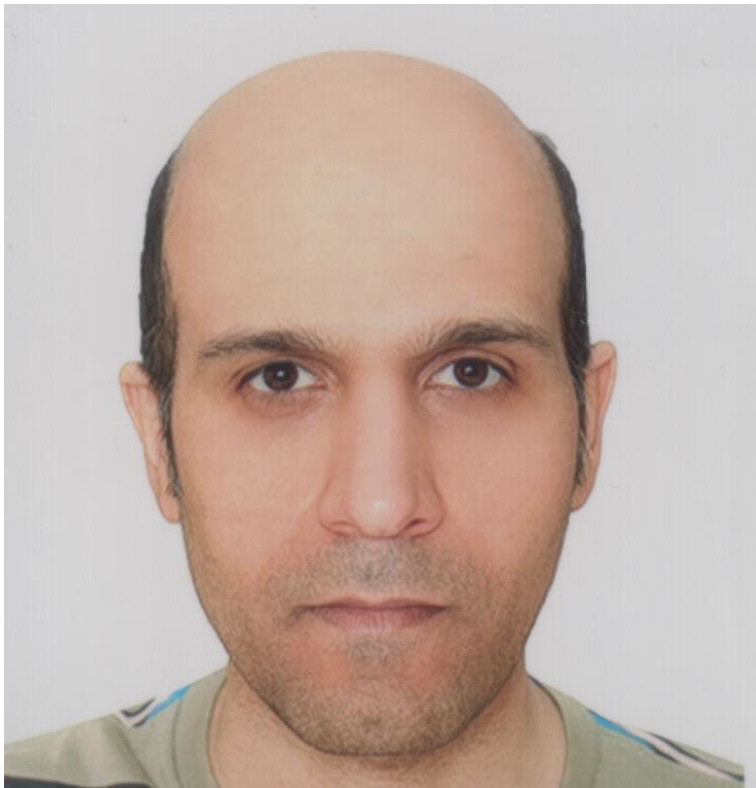
\includegraphics[width=6cm]{cropped_010_5}};
            \end{tikzpicture}
        \end{center}
        \vspace{.3cm}
        %%%%%%%%%%%%%%%%%%%%%%%%%%%%%%%%%%%%%%%%%%%%%%%%%%%%
        % YOUR PERSONAL INFROMATION
        \phantomsection{}
        \addcontentsline{toc}{section}{Kontakte} % Personal info
        \section*{\Large Kontakte}
        \begin{tabularx}{\textwidth}{cY}
            \faPhone{}      & \href{tel:+49 176 703 552 53}{+49 176 703 552 53} \\
            \faSkype{}      & \href{skype:Morteza Montahaee?chat}{Morteza Montahaee} \\
            \faEnvelope{}   & \href{mailto:morteza.montahaee@rwth-aachen.de}{\fontsize{9.4}{12}\selectfont morteza.montahaee@rwth-aachen.de} \\
            \scalebox{1.144}{\faMapMarker}{}  & \href{https://www.bing.com/maps?q=Otto+str+19+aachen\&FORM=AWRE}{Ottostr. 19, 52070 Aachen} \\
        \end{tabularx}
        \vspace{.3cm} \\
        \rule{\linewidth}{0.4pt} \\
        %%%%%%%%%%%%%%%%%%%%%%%%%%%%%%%%%%%%%%%%%%%%%%%%%%%%%%%%%
        % YOUR LINKS, YOU MAY ALSO ADD A PERSONAL WEBSITE OR PORTFOLIO
        \phantomsection{}
        \addcontentsline{toc}{section}{Links}
        \section*{\large Links}
        \begin{tabular}{cl}
        %    \faCode{}     & \href{https://example.com}{example.com}
            \faGithub{}   & \href{https://github.com/montahaee}{montahaee} \\
            \faGlobe{} & \href{https://montahaee.github.io/}{montahaee.github.io} \\
            % \faXing{}     & \href{https://www.xing.com/profile/Mor_Mon7373990/cv}{/Mor\_Mon7373990} \\
            
\includegraphics[width=1.25em]{icon-twitterx-500.png} &  \href{https://x.com/Mor_Montahaee}{Mor\_Montahaee} \\
        \end{tabular}
        \vspace{10pt} \\
        \rule{\linewidth}{0.4pt} \\
        %%%%%%%%%%%%%%%%%%%%%%%%%%%%%%%%%%%%%%%%%%%%%%%%%%%%%%%%%%%%
        % YOUR SKILLS
        % Add/Remove as seen fit, Icons: https://packages.oth-regensburg.de/ctan/fonts/fontawesome5/doc/fontawesome5.pdf
        \phantomsection{}
        \addcontentsline{toc}{section}{Skills}
        \section*{\large Skills}
        %%%%%%%%%%%%%%%%%%%%%%%%%%%%%%%%%%%%%%%%%%%%%%%%%%%%%%%%%%%%%%%%
        % GRADESCALE (if nesseary, e.g. if you apply abroad, where scales
        % are different. You should at least provide, what the best possible
        % grade and what the worst possible grade is)
        \begin{center}
            \begin{tikzpicture}
                % Mid-level
                \draw[fill=green!70!black] (0,0) circle (0.75ex);
                \node[left] at (-0.25,0) {\betiny Gut};

                % High-level
                \draw[fill=red!50!white] (0.5,1.0) circle (0.75ex);
                \node[right] at (0.75,1.0) {\betiny Sehr Gut};

                % Low-level
                \draw[fill=magenta!45!white] (1.0,0) circle (0.75ex);
                \node[right] at (1.25,0) {\betiny Grundkenntnisse};
            \end{tikzpicture}
        \end{center}

        \begin{tabularx}{\textwidth}{cY}
            \faCode{}        & {\textcolor{green!75!black}{C++}}, {\textcolor{green!75!black}{C}}, {\textcolor{red!45!white}{Python}}, {\textcolor{magenta!40!white}{Bash}}, {\textcolor{green!75!black}{PHP}}, {\textcolor{green!75!black}{Javascript}}, {\textcolor{red!45!white}{C\#}}, {\textcolor{red!45!white}{Java}}, {\textcolor{green!75!black}{MariaDB}}, {\textcolor{green!75!black}{MySQL}}, {\textcolor{magenta!40!white}{Visual Basic}} \\
            \faPen*{}        & {\textcolor{red!45!white}{\LaTeX}}, {\textcolor{red!45!white}{Liquid}}, {\textcolor{red!45!white}{HTML}}, {\textcolor{green!75!black}{CSS}}, {\textcolor{magenta!40!white}{SHACL}} \\
            \faFont{}        & \{MS, Libre\} Office, Vim, PDF-XChange,  Adobe Acrobat \\
            \faCogs{}        & Dual (Windows, Linux) \\
            \faLaptopCode{}  & IntelliJ, Rider, Visual Studio/Code, PyCharm,  CLion, DataGrip, MATLAB\\
            \faToolbox{}     & Docker, Enterprise Architect, Git
        \end{tabularx}
        \vspace{1pt} \\
        \rule{\linewidth}{0.4pt}

        \vfill
%        {\tiny GPA: (1) very good $\approx$91\%-100\%, (2) good $\approx$81\%-90\%, (3) satisfactory $\approx$66\%-80\%, (4) sufficient $\approx$50\%-65\%, (5) failed $\approx$0\%-49\%}
        \phantomsection{}
        \begin{center}
            {\tiny \textbf{GPA}: (18-20) sehr gut $\approx$90\%-100\%, (15-17) gut $\approx$80\%-89\%, (12-14) befriedigend $\approx$70\%-79\%, (10-12) ausreichend $\approx$60\%-69\%, (0-9) mangelhaft $\approx$0\%-59\%\label{ft:gpasystem}}
%            \href{https://en.wikipedia.org/wiki/Academic_grading_in_Iran}{\scalebox{0.72}{\faExternalLink}}
            \externallink{https://en.wikipedia.org/wiki/Academic_grading_in_Iran}{0.72}{0.25}{-0.15}{0}
        \end{center}
    \end{minipage}
}
\hfill
\fcolorbox{red}{mainbg}{%
    \begin{minipage}[t][\dimexpr\textheight-2\fboxrule-2\fboxsep\relax][t]{\dimexpr0.6\textwidth-2\fboxrule-2\fboxsep\relax}
        \color{maintext}
        \vspace{3pt}
        %%%%%%%%%%%%%%%%%%%%%%%%%%%%%%%%%%%%%%%%%%%%%%%%%%%%%%%%%%%
        % EDUCATION
        \phantomsection{}
        \addcontentsline{toc}{section}{Ausbildung} %Education/Ausbildung
        \section*{\scshape\Large Ausbildung \rule{\linewidth}{0.4pt}} \vspace{-7pt}
%
        {\large \textbf{Angewandte Mathematik und Informatik (\href{https://montahaee.github.io/assets/pdf/de/apply/Abschlussbescheinigung.pdf}{\textcolor{cyan!60!black}{\fontsize{11.15pt}{13pt}\selectfont Abschluss{\externallink{}{0.62}{1.25}{-0.43}{10}}}})}} \\[1ex]
        \faUniversity{} FH Aachen, University of Applied Sciences \\
%        {\scshape\fontseries{light}\selectfont\footnotesize \faMapMarker{} Jülich \qquad{} \faCalendar{} Okt 2019 \textendash{} Sep 2024} \\
        \eduevent{Jülich}{Okt 2019}{Sep 2024}
%        {\href{https://montahaee.github.io/assets/pdf/de/apply/Abschlussbescheinigung.pdf}{\textcolor{cyan!70!black}{Studiengang}}: Bachelor of Science} \\[1ex]
        {Studiengang}{Bachelor of Science}{.1cm}
        {Note: 2.7} \\[0ex]
%        {\footnotesize Subsidiary subject: Psychology} \\
        {\footnotesize \textbf{Schwerpunkt}: Analysis, Lineare Algebra, Stochastik, Numerik, Algorithmen und Datenstrukturen, Data Science, Datenbanken, Softwaretechnik} \\
        {\footnotesize \href{https://montahaee.github.io/assets/pdf/de/projects/myFH_Bachelorthesis.pdf}{\textcolor{cyan!70!black}{Bachelorarbeit\externallink{}{0.62}{1.35}{-0.3}{0}}}: Datengetriebene äu\ss{}ere Differentialrechnung auf Graphen zur Diskretisierung von elliptischen partiellen Differentialgleichungen} \\[2ex]

        {\large \textbf{Mathematik (Ohne Abschluss)}} \\[1ex]
        \faUniversity{} RWTH University \\
        \eduevent{Aachen}{Okt 2012}{Sep 2019}
        {Studiengang}{Master of Science}{.1cm}  \vspace{-10pt}
        {} \\
        {\footnotesize Abgschlossene Module: \href{https://montahaee.github.io/assets/pdf/de/apply/bild\_verarbeitung\_zeugnis.pdf}{\textcolor{cyan!70!black}{Bildverarbeitung{\externallink{}{0.62}{1.25}{-0.33}{10}}}}, \href{https://montahaee.github.io/assets/pdf/de/apply/neuro_science.pdf}{\textcolor{cyan!70!black}{Neuroscience{\externallink{}{0.62}{1.25}{-0.33}{10}}}}, Numerik (PDE),
            \href{https://montahaee.github.io/assets/pdf/de/apply/optimierungc_zeugnis.pdf}{\textcolor{cyan!70!black}{Optimierungstheorie{\externallink{}{0.62}{-0.25}{-0.33}{-80}}}}, Variationsrechnung} \\[1ex]
        {\large \textbf{Spracherwerb}} \\[1ex]
        \faUniversity{} Sprachenzentrum der RWTH \\
%        {\scshape\fontseries{light}\selectfont\footnotesize New York \qquad Sep 2005 \textendash{} Jun 2010} \\
        \eduevent{Aachen}{Apr 2011}{Jun 2012}{Abschluss}{\href{https://de.wikipedia.org/wiki/Deutsche_Sprachpr\%C3\%BCfung_f\%C3\%BCr_den_Hochschulzugang}{\textcolor{cyan!70!black}{DSH{\externallink{}{0.62}{.75}{0.08}{10}}}}}{.575cm}
%        {Degree: Secondary school leaving certificate} \\[1ex]
        \vspace{-5pt}
        {}\\
        {Note: \href{https://montahaee.github.io/assets/pdf/de/apply/sprach_zeugnis.pdf}{\textcolor{cyan!70!black}{Stufe II{\externallink{}{0.62}{.75}{0.08}{10}}}}} \\[1ex]
%        {\footnotesize Elective Courses: Chemistry, Engineering, Art} \\
%        \vspace{-3pt}
        {\large \textbf{Angewandte Mathematik (\href{https://montahaee.github.io/assets/pdf/en/apply/bsc_degree.pdf}{\textcolor{cyan!60!black}{Abschluss{\externallink{}{0.62}{1.25}{-0.3}{0}}}})}} \\
        \faUniversity{} \href{https://en.wikipedia.org/wiki/Payame_Noor_University}{\textcolor{green!30!black}{Payame Noor}} University{\textcolor{green!30!black}{\externallink{https://en.wikipedia.org/wiki/Payame_Noor_University}{0.82}{1.25}{-0.23}{0}}}
        \eduevent{Pakdasht}{Okt 2005}{Jul 2009}{Studiengang}{Bachelor of Science}{.1cm}
        {Note: 15.54\hyperref[ft:gpasystem]{\textcolor{cyan!60!black}{$^{\text{\tiny \textbf{GPA}}}$\internallink{}{.75}{-1.05}{-.95}{0}}}} \\[1ex]
        {\footnotesize \textbf{Schwerpunkt}: Lineare/ Algebra, Numerische (ODE) und Mathematische Analysis, Mathematische Statistik, Graphentheorie, Mathematische Modelle der Natur (ODE)} \\
        {\footnotesize Bachelorarbeit: Anwendung Nichtlinear Konjugierte Gradient-Algorithmen zur Abschätzung elektromagnetischer Inversion} \\[2ex]
         \vspace{+2pt}
        %%%%%%%%%%%%%%%%%%%%%%%%%%%%%%%%%%%%%%%%%%%%%%%%%%%%%%%%%%
        % WORK EXPERIENCE
        \phantomsection{}
        \addcontentsline{toc}{section}{Berufliche Erfahrung}   % Work Experience
        \section*{\scshape\Large Berufliche Erfahrung \rule{\linewidth}{0.4pt}} \vspace{-7pt}
%
        \faUniversity{} {\large \textbf{\href{https://dap-aachen.de/}{
            \textcolor{green!30!black}{DAP}} RWTH{\textcolor{green!30!black}{\externallink{https://dap-aachen.de/}{0.82}{1.0}{0.1}{0}}}}} \\
        {{\fontseries{medium}\selectfont Vollzeit, \href{https://de.wikipedia.org/wiki/Mathematisch-technischer_Softwareentwickler}{
            \textcolor{green!30!black}{MATSE}}-Azubi{\textcolor{green!30!black}{\externallink{https://de.wikipedia.org/wiki/Mathematisch-technischer_Softwareentwickler}{0.82}{0.9}{0.1}{0}}}}} \\
        {\faCalendar {} {\scshape\fontseries{light}\selectfont\footnotesize Okt 2019 \textendash{} Aug 2023}}
        \vspace{+5pt}
        \begin{itemize}
            \setlength{\itemsep}{-3pt}
%            \item Durchführung verschiedener Aufgaben
%            \begin{itemize}
                \item[\larrow{bgcol}]\href{https://montahaee.github.io/assets/pdf/en/projects/praxisbericht2_morteza_montahaee_signed.pdf}{\textcolor{darkgreen!70!red}{Entwicklung{{\externallink{}{0.62}{1.25}{-0.43}{0}}}}}einer \href{https://plm.sw.siemens.com/de-DE/nx/}{\textcolor{cyan!70!black}{NX{\textcolor{cyan!70!black}{\externallink{https://plm.sw.siemens.com/de-DE/nx/}{0.62}{1.55}{-0.43}{0}}}}}CAD Bibliothek zur Generierung von Lattice
                in C\#, wodurch die Effizienz der Datentransfers und die Leistungsfähigkeit bei der Verarbeitung komplexer Strukturen verbessert wurden
                \item[\larrow{bgcol}]\href{https://montahaee.github.io/assets/pdf/en/projects/praxisbericht1_morteza_montahaee_signed.pdf}{\textcolor{darkgreen!70!red}{Entwurf{{\externallink{}{0.62}{1.65}{-0.33}{0}}}}}von Workflow-Management additiver Prozesse (\href{https://dap-aachen.de/2022-06-22-idam}{\textcolor{cyan!70!black}{IDAM\externallink{}{0.62}{1.65}{-0.33}{0}}}) mit Enterprise Architect (\href{https://sparxsystems.com/}{\textcolor{cyan!70!black}{EA\externallink{}{0.62}{1.5}{-0.33}{0}}}) zur präziseren Prozesssteuerung und verbesserten Nachvollziehbarkeit
                \item[\larrow{bgcol}] \href{https://montahaee.github.io/assets/pdf/de/apply/recommandation_letter.pdf}{\textcolor{darkgreen!70!red}{Beteiligung{{\externallink{}{0.62}{1.25}{-0.33}{0}}}}} an der Entwicklung von Forschungsdatenmodellen mit Python (auf \href{https://www.itc.rwth-aachen.de/cms/it-center/services/forschung/~smhwy/coscine/}{\textcolor{cyan!70!black}{{Coscine{\externallink{}{0.62}{1.25}{-0.33}{0}}}}}), was die Effizienz und Konsistenz bei der Verwaltung gro\ss er wissenschaftlicher Datensätze erhöhte
                \item[\larrow{bgcol}]Unterstützung der Firma MAT.TRAFFIC GmbH im Rahmen einer MATSE \href{https://blog.rwth-aachen.de/itc/en/2017/04/12/software-engineering-messe-der-matse2015} {\textcolor{cyan!70!black}{Projektarbeit\externallink{}{0.62}{1.5}{-0.33}{0}}}in Python: Geo-Erkennung von Kreuzungen für intelligente Verkehrssysteme und Stadtplanung mithilfe der Metadaten von OpenStreetMap(\href{https://www.openstreetmap.org/}{\textcolor{cyan!70!black}{OSM\externallink{}{0.62}{1.5}{-0.33}{0}}}), was zur Automatisierung der Erkennung urbaner Kreuzungen und zur Verbesserung der Planungsprozesse beitrug
            \end{itemize}
%            \item Other Task
%        \end{itemize}
%
%        \faUniversity{} {\large \textbf{\href{https://dap-aachen.de/}{
%            \textcolor{green!30!black}{DAP}} RWTH \externallink{https://dap-aachen.de/}{0.63}{true}}} \\
%        {{\fontseries{medium}\selectfont Vollzeit, \href{https://de.wikipedia.org/wiki/Mathematisch-technischer_Softwareentwickler}{
%            \textcolor{green!30!black}{MATSE}}-Azubi \externallink{https://de.wikipedia.org/wiki/Mathematisch-technischer_Softwareentwickler}{0.72}{true}}} \\
%        {\faCalendar {} {\scshape\fontseries{light}\selectfont\footnotesize Okt 2019 \textendash{} Aug 2023}}
%        \begin{itemize}
%            \setlength{\itemsep}{-3pt}
%            \item Durchführung verschiedener Aufgaben
%            \begin{itemize}
%                \item[\larrow{bgcol}]
%                \item and more Stuff
%            \end{itemize}
%            \item Other Task
%            \begin{itemize}
%                \item That included more Stuff
%                \item and other more different Stuff
%            \end{itemize}
%            \item tellus elementum sagittis vitae et
%            \item aliquam sem et tortor consequat
%            \item ullamcorper velit sed ullamcorper morbi tincidunt
%            \item rhoncus est pellentesque elit ullamcorper dignissim
%        \end{itemize}
%%
%        {\large \textbf{ACME Corp}}\\
%        {{\fontseries{medium}\selectfont Traineeship, Occupation}}\\
%        {\scshape\fontseries{light}\selectfont\footnotesize Aug 2010 \textendash{} Oct 2013}
%        \begin{itemize}
%            \setlength{\itemsep}{-4pt}
%            \item massa tempor nec feugiat nisl pretium fusce id
%        \end{itemize}
        \vfill%
        {\hfill\small\fontseries{extralight}\selectfont Seite \thepage\, von  \pageref{LastPage}\hfill}
    \end{minipage}
}%

\newpage
%%%%%%%%%%%%%%%%%%%%%%%%%%%%%%%%%
% PAGE 2
%%%%%%%%%%%%%%%%%%%%%%%%%%%%%%%%%
\fcolorbox{red}{mainbg}{%
    \begin{minipage}[t][\dimexpr\textheight-2\fboxrule-2\fboxsep\relax][t]{\dimexpr0.6\textwidth-2\fboxrule-2\fboxsep\relax}
        \color{maintext}
         \vspace{.2cm}
        %%%%%%%%%%%%%%%%%%%%%%%%%%%%%%%%%%%%%%%%%%%%%%%%
        % PROFILE
        \phantomsection{}
        \addcontentsline{toc}{section}{Profil} % Profile
        \section*{\scshape{\fontsize{12.65}{15}\selectfont Profil} \rule{\linewidth}{0.4pt}}

        Absolvent in Angewandter Mathematik und Informatik mit umfangreicher Erfahrung in der Softwareentwicklung mit einem Fokus auf \href{https://de.wikipedia.org/wiki/Geometrische_Modellierung#Generative_Modellierung}{\textcolor{cyan!70!black}{Generative{\externallink{}{0.62}{.75}{0.08}{10}}}} Modellierung, Datenbankmanagement, Data Science und Webentwicklung. Leidenschaft für mathematische Methoden zur Lösung komplexer Probleme und ihrer Implementierung möglichst nach \href{https://de.wikipedia.org/wiki/Entwurfsmuster}{\textcolor{cyan!70!black}{Entwurfsmuster{\externallink{}{0.62}{1.25}{-0.73}{10}}}}prinzipien.
        \vspace{.75cm}
        %%%%%%%%%%%%%%%%%%%%%%%%%%%%%%%%%%%%%%%%%%%%%%%%
        % PROJECTS /other activities
        \phantomsection
        \addcontentsline{toc}{section}{Weitere berufliche Tätigkeiten}   % Further Work Experience
%        \section*{\scshape\Large Weitere berufliche Tätigkeiten \rule{\linewidth}{0.4pt}}
%        \section*{\scshape\large Weitere berufliche Tätigkeiten \rule[0ex]{3.475cm}{0.4pt}}
        \section*{\scshape{\fontsize{12.65}{15}\selectfont Weitere berufliche Tätigkeiten} \rule[0ex]{\linewidth}{0.4pt}}

        \begin{justify}
        \setlength{\parindent}{0pt}
        \faBuilding{} {\normalsize \textbf{Event Probat}} \\[1ex]
        \jobevent{Aachen}{Nov 2014}{Sep 2019}{Kellner und Eventassistent}{3.425cm} \\
        \faIndustry{} {\normalsize \textbf{Frankenberg}} \\[1ex]
        \jobevent{Würselen}{Jul 2012}{Okt 2014}{Aushelfer}{6.4cm} \\
        \faGopuram{} {\normalsize \textbf{NAJA}} \\[1ex]
        \jobevent{Teheran}{Aug 2009}{Feb 2011}{Wehrdienst}{6.cm} \\
        \vspace{+2pt}
        \end{justify}

%        \faM{\scshape\fontseries{light}\selectfont\footnotesize Acme Corp \qquad 2017} \\
%        Lorem ipsum dolor sit amet, consectetur adipiscing elit, sed do eiusmod tempor incididunt ut labore et dolore magna aliqua. Tincidunt praesent semper feugiat nibh sed pulvinar. Tristique nulla aliquet enim tortor at auctor. \\[1ex]
%        Skill 1, Skill 2, Skill 3 \\
%
%        {\large \textbf{Lacus laoreet non}} \\
%        {\scshape\fontseries{light}\selectfont\footnotesize Acme Corp \qquad 2018} \\
%        Pellentesque elit ullamcorper dignissim cras tincidunt. Sit amet commodo nulla facilisi nullam vehicula ipsum. Blandit cursus risus at ultrices mi tempus imperdiet. Lectus sit amet est placerat in egestas erat.\\[1ex]
%        Skill 1, Skill 2, Skill 3, \LaTeX \\
%
%        {\large \textbf{Viverra maecenas accumsan lacus}} \\
%        {\scshape\fontseries{light}\selectfont\footnotesize Private \qquad 2022 and ongoing} \\
%        Quisque non tellus orci ac auctor augue mauris augue neque. Sit amet luctus venenatis lectus magna fringilla urna porttitor rhoncus. Proin nibh nisl condimentum id venenatis a condimentum vitae sapien. \\[1ex]
%        Skill 1, Skill 2, Skill 3 \\
%
%        {\large \textbf{Ut faucibus pulvinar elementum}} \\
%        {\scshape\fontseries{light}\selectfont\footnotesize TU Dresden \qquad 2022} \\
%        Proin nibh nisl condimentum id venenatis a condimentum vitae sapien. Amet aliquam id diam maecenas ultricies mi eget. Viverra maecenas accumsan lacus vel facilisis volutpat. \\[1ex]
%        Skill 1, Skill 2, Skill 3 \\


%        \begin{minipage}{\textwidth}
%            \begin{tabular}{@{}p{0.4\textwidth} p{0.45\textwidth}@{}}
%                \cvdetail{Kellner und Eventassistent\hspace{22.5120em}\textcolor{magenta!60!black}{11/2014 - 09/2019}}\\
%                \cvdetail{{Aushelfer\hspace{28.7em}\textcolor{green!40!black}{07/2012 - 10/2014}}}\\
%                \cvdetail{{Wehrdienst\hspace{27.605em}\textcolor{red!50!black}{08/2009 - 02/2011}}}\\
%            \end{tabular}
%        \end{minipage}

%        {\large \textbf{Quisque non tellus orci}} \\
%        {\scshape\fontseries{light}\selectfont\footnotesize ACME Corp. \qquad 2023} \\
%        Viverra maecenas accumsan lacus vel facilisis volutpat. Tortor condimentum lacinia quis vel eros donec ac odio tempor. Ultricies lacus sed turpis tincidunt id aliquet risus. \\[1ex]
%        Skill 1, Skill 2, Skill 3 \\
%
%        {\large \textbf{Amet consectetur adipiscing elit}} \\
%        {\scshape\fontseries{light}\selectfont\footnotesize ACME Corp \qquad 2023} \\
%        Eget lorem dolor sed viverra. Eleifend donec pretium vulputate sapien. Pellentesque pulvinar pellentesque habitant morbi tristique senectus et netus et. Augue neque gravida in fermentum et. Ullamcorper velit sed ullamcorper morbi tincidunt ornare massa eget egestas. \\[1ex]
%        Skill 1, Skill 2, Skill 3 \\
%
%        {\large \textbf{Augue neque gravida in fermentum}} \\
%        {\scshape\fontseries{light}\selectfont\footnotesize Sample Uni \qquad 2023} \\
%        met aliquam id diam maecenas ultricies mi eget. Viverra maecenas accumsan lacus vel facilisis volutpat. Tortor condimentum lacinia quis vel eros donec ac odio tempor. Ultricies lacus sed turpis tincidunt id aliquet risus. \\[1ex]
%        Skill 1, Skill 2, Skill 3, \LaTeX

        \vfill%
        {\hfill\small\fontseries{extralight}\selectfont Seite \thepage\, von \pageref{LastPage}\hfill}
    \end{minipage}
}
\hfill%
\fcolorbox{red}{sidebg}{%
    \begin{minipage}[t][\dimexpr\textheight-2\fboxrule-2\fboxsep\relax][t]{\dimexpr0.4\textwidth-2\fboxrule-2\fboxsep\relax}
        \color{sidetext}
        % \vspace{.5cm}
        %%%%%%%%%%%%%%%%%%%%%%%%%%%%%%%%%%%%%%%%%%%%%%%%%%%%%%%%
        % YOUR NAME AND PREFERED PRONOUS AGAIN AS HEADER
        {\bfseries\scshape\HUGE Morteza} \\
        {\bfseries\scshape\huge Monthaee} \qquad {\large\textbf{ Lebenslauf}}
        \vspace{.3cm} \\
        %%%%%%%%%%%%%%%%%%%%%%%%%%%%%%%%%%%%%%%%%%%%%%%%%%%%%%%%%%
        % LANGUAGES
        \phantomsection
        \addcontentsline{toc}{section}{Sprachen} %  Languages
        \section*{\large Sprachen}
        \begin{tabular}{cl}
            \faLanguage{} & Deutsch (Verhandlungssicher) \\
            \faLanguage{} & English ({\fontsize{9.25}{12}\selectfont Flie\ss end in Wort und Schrift}) \\
            \faLanguage{} & Persisch (Muttersprache) \\
            \faLanguage{} & Arabisch ({\fontsize{9.25}{12}\selectfont Erweiterte Grundkenntnisse})
        \end{tabular}
        \vspace{.3cm}
        \\
        \rule{\linewidth}{0.4pt}
        \\
        %%%%%%%%%%%%%%%%%%%%%%%%%%%%%%%%%%%%%%%%%%%%%%%%%%%%%%%%%%%%
        % CERTIFICATES AND AWARDS RECEIVED or any other things that you find important
        \phantomsection
        \addcontentsline{toc}{section}{Interesse}   % Certificates and Prizes
        \section*{\large Interesse}
%        \begin{tabularx}{\textwidth}{cY}
%%            2010 & Etiam tempor orci eu \\
%%            2010 & Quam nulla porttitor massa \textemdash{} 3\textsuperscript{rd} place \\
%%            2011 & Quis imperdiet massa tincidunt \textemdash{} 3\textsuperscript{rd} place \\
%%            2016 & Vestibulum sed arcu non odio euismod \\
%%            2016 & Non enim praesent elementum facilisis \\
%%            2016 & Blandit libero volutpat sed cras \\
%%            2016 & Eget dolor morbi non arcu \\
%            & Variationsrechnung     \\
%            & Differenzialgeometrie  \\
%            & Data Science            \\
%            & Design Patterns         \\
%        \end{tabularx}
        \begin{tabular}{cl}
            
\includegraphics[width=1.25em]{square-root-variable-solid} & Variationsrechnung \\
            
\includegraphics[width=1.25em]{geometry_1} & Differenzialgeometrie \\
            
\includegraphics[width=1.25em]{chart-line-solid} & Data Science \\
            
\includegraphics[width=1.25em]{rangoli} & Design Patterns \\
        \end{tabular}
        \vspace{.3cm}
        \\
        \rule{\linewidth}{0.4pt}
        \\
        %%%%%%%%%%%%%%%%%%%%%%%%%%%%%%%%%%%%%%%%%%%%
        % HOBBIES
        % Change Icons here https://packages.oth-regensburg.de/ctan/fonts/fontawesome5/doc/fontawesome5.pdf
        \phantomsection
        \addcontentsline{toc}{section}{Hobbys}  % Hobbies
        \section*{\large Hobbys}
        \begin{tabularx}{\textwidth}{cY}
            
\includegraphics[width=1.25em]{wrestling1} & Ringen \\
            
\includegraphics[width=1.25em]{football} & Fu\ss ball \\
            
\includegraphics[width=1.25em]{hiking} & Wandern \\
            
\includegraphics[width=1.25em]{history_scroll} & Geschichte \\
            
\includegraphics[width=1.275em]{math2} & Mathematik \\
        \end{tabularx}
        \vspace{.3cm}
        \\
        \rule{\linewidth}{0.4pt}
    \end{minipage}%
}%
%    \cleardoubleemptypage
% \afterpage{\null\newpage}
\end{document}